
\documentclass[12pt]{article}

% margin left and right with \setlength{\itemindent}{-.5in} %
\usepackage{enumitem}

% leave out section numbers in subsection numbering %
\usepackage[T1]{fontenc}
\renewcommand*\thesubsection{\arabic{subsection}}

% include Roman numerals for sections %
\renewcommand{\thesection}{\Roman{section}}
%Roman numerals for subsections like this \renewcommand{\thesubsection}{\Roman{subsection}}%
% include the pckage of the color%
\usepackage[usenames, dvipsnames]{color}
\usepackage[english]{babel}
\usepackage[utf8x]{inputenc}
\usepackage{amsmath}
\usepackage{graphicx}
\usepackage{subfiles}

%define your own color %
\definecolor{mygray}{gray}{0.9}
\begin{document}
	\listoffigures
	\title{Chapter 3 : Conception}
	\maketitle
	
	\section{Introduction}

	\section{Modeling Language}
		A modeling language is used to describe a system, a standard or methodology, general or domain-specific and / or context based on its components and relationships.
	There are several modeling languages, the best known are UML and Merise. In our project we chose UML as Modeling language.
	\\
	UML is a Unified Modeling language that can can model a problem in a standard way.
	\\
	\\
	\textbf{Why UML ?}
	We chose UML for these reasons : 
	\begin{itemize}
	\item To obtain a very high level modeling independent of the language and environments
	\item Document a project. 
	\end{itemize}
	
	\section{Global Conception}
	In this section, we highlight the architecture of our application, we starting  with physical architecture and the logical architecture.
	\subsection{Physical Architecture}
	It is primordial to designing any computer system to choose the model architecture that will be adequate to ensure proper functioning, performance, the reuse and reliable interconnection of this system with others. We opt for this purpose for the physical architecture described in the figure below.
	\begin{figure}[h]
		\centering
		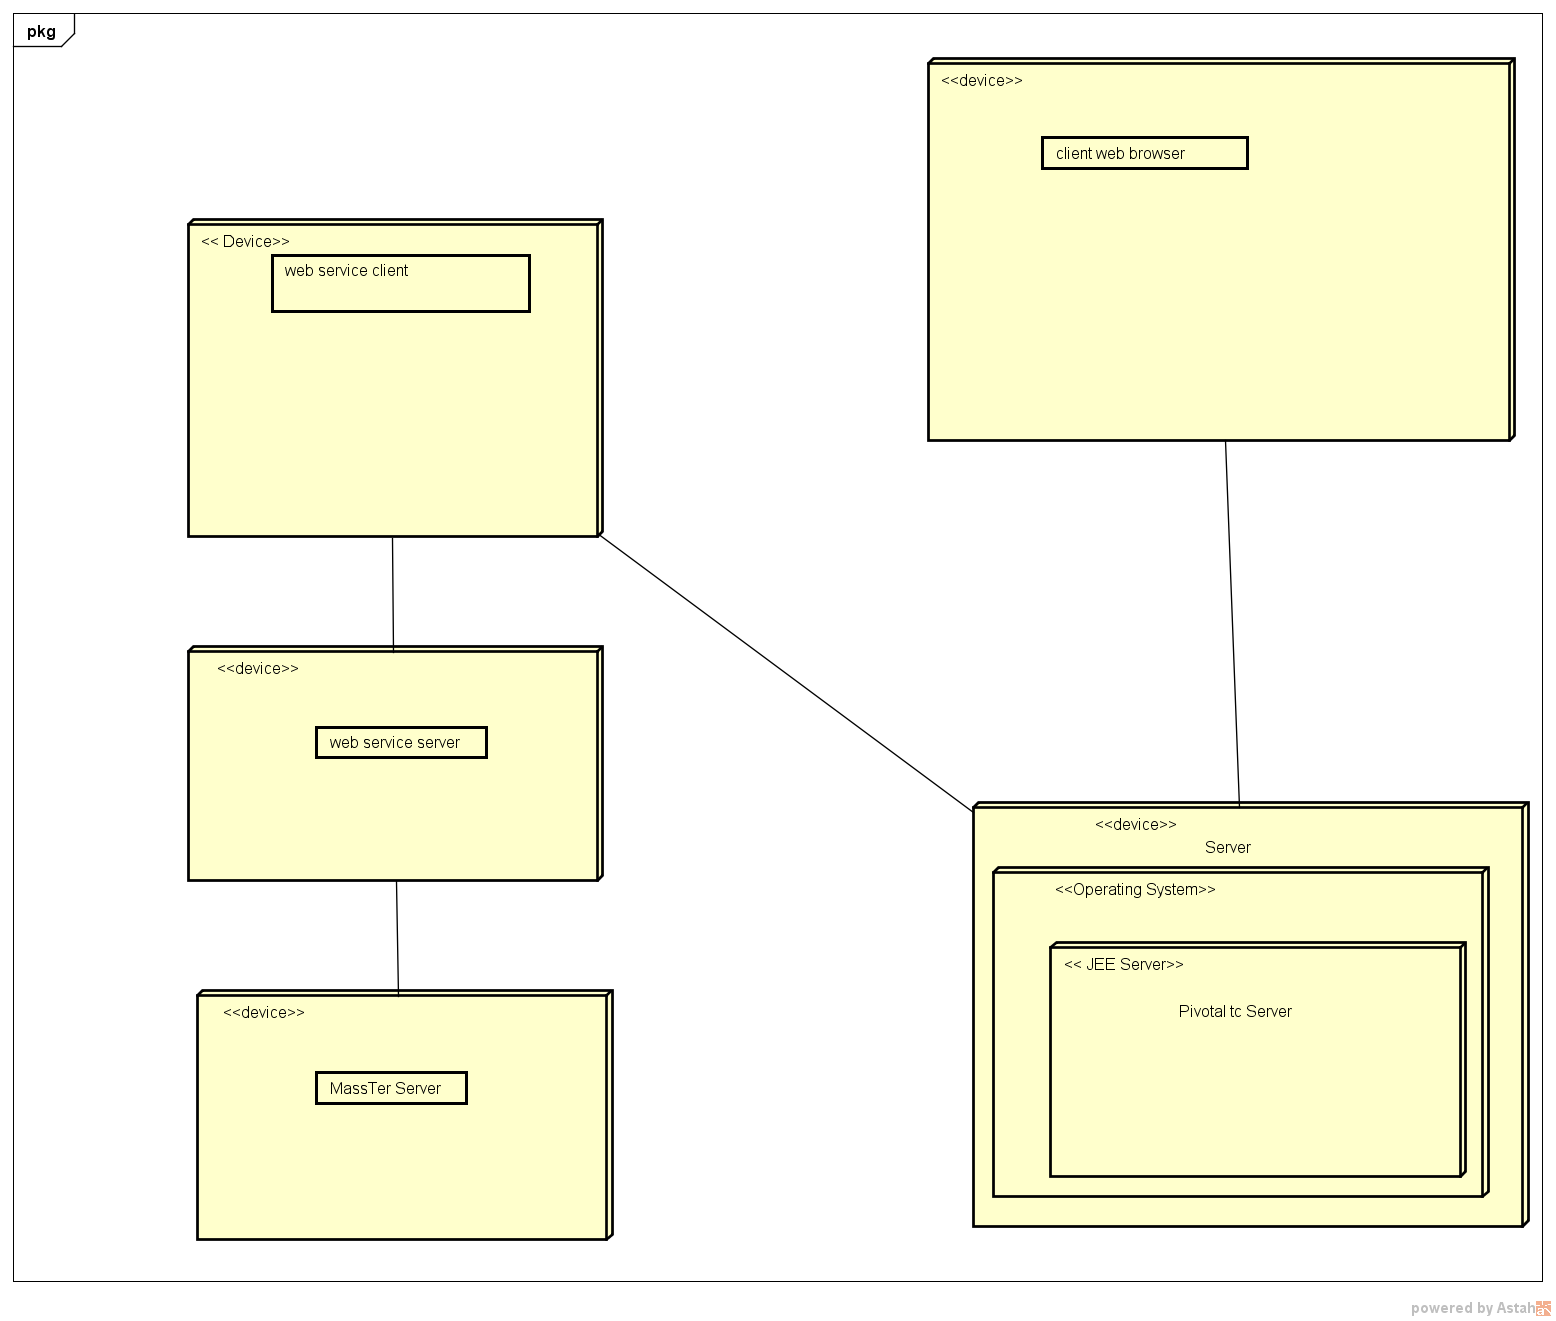
\includegraphics[width=1\textwidth]{DeploymentDiagramPhysicalArchitecture.png}
		\caption{Deployment Diagram Physical Architecture}
	\end{figure}    
	\subsection{Logical Architecture}
	\subsection{Design Pattern}
	\section{Detailed Conception}
	\subsection{Package Diagram}
	\subsection{Class Diagram}
	\subsection{Sequence Diagram}
	\section{Conclusion}
	
\end{document}